% Classification of DAE optimization strategies.
%
% Re-authored from Biegler (2010), Figure 8.10, printed p. 245, in Section 8.6
% "Numerical Methods Based on NLP Solvers" (pp. 244-247). It replaces
% media/dynamic_optimization_strategies.png, which was a SCREENSHOT of that
% figure -- unreadable when scaled, uneditable, and not greyscale-checkable.
%
% The two top-level branches are Biegler's own names for them, p. 244:
% "Optimize then Discretize" (the indirect / variational approach) and
% "Discretize then Optimize" (the direct NLP approach). The three arrow labels
% are his: "discretize controls" onto Sequential, "discretize all variables"
% onto Direct transcription, and multiple shooting reached from BOTH sides --
% p. 245, "Optimization with multiple shooting serves as a bridge between
% sequential and direct transcription approaches".
%
% GREYSCALE. Every box is white with a black rule; the two top-level branches
% are told apart by the arrow's linestyle (solid = optimize-then-discretize,
% dashed = discretize-then-optimize) and by their labels, never by colour.

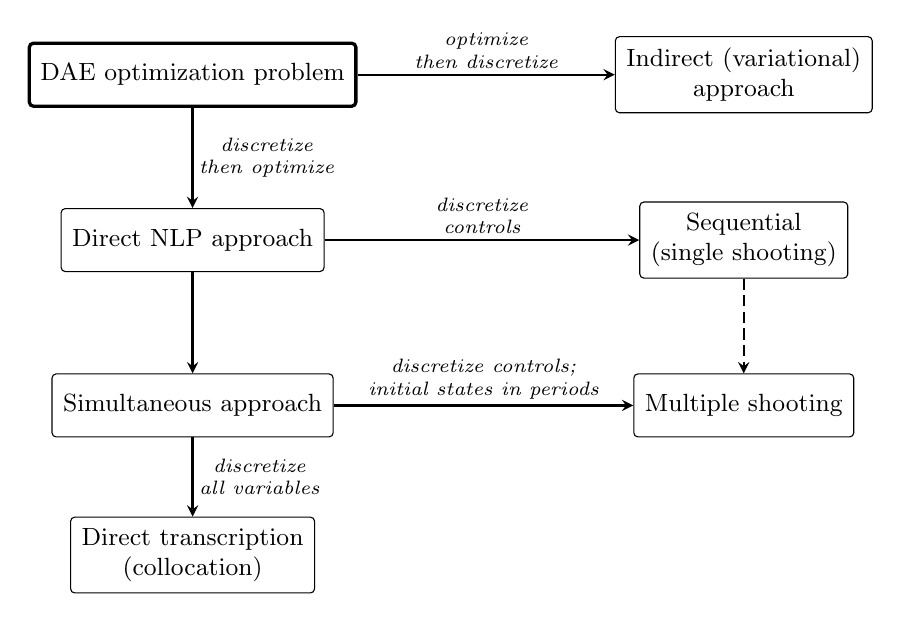
\begin{tikzpicture}[
  node distance = 8mm,
  every node/.style = {font=\small},
  box/.style = {draw, rectangle, rounded corners=1.5pt, align=center,
                fill=white, inner sep=4pt, minimum height=8mm},
  root/.style = {box, very thick},
  lbl/.style  = {font=\scriptsize\itshape, align=center, inner sep=2pt},
  go/.style   = {->, >=stealth, thick},
  bridge/.style = {->, >=stealth, thick, dash pattern=on 4pt off 2pt},
]

% No \ref/\eqref anywhere in this file: it is rendered standalone by the
% Makefile as well as \input by the handout, and a cross-reference would come
% out as "??" in the standalone build.
\node[root] (dae) at (0,0) {DAE optimization problem};

% --- Optimize then discretize -------------------------------------------
\node[box] (ind) at (7.0,0) {Indirect (variational)\\ approach};
\draw[go] (dae) -- node[lbl, above] {optimize\\ then discretize} (ind);

% --- Discretize then optimize -------------------------------------------
\node[box] (nlp) at (0,-2.1) {Direct NLP approach};
\draw[go] (dae) -- node[lbl, right] {discretize\\ then optimize} (nlp);

\node[box] (seq) at (7.0,-2.1) {Sequential\\ (single shooting)};
\draw[go] (nlp) -- node[lbl, above] {discretize\\ controls} (seq);

\node[box] (sim) at (0,-4.2) {Simultaneous approach};
\draw[go] (nlp) -- (sim);

\node[box] (ms) at (7.0,-4.2) {Multiple shooting};
\draw[go] (sim) -- node[lbl, above] {discretize controls;\\ initial states in periods} (ms);
\draw[bridge] (seq) -- (ms);

\node[box] (dt) at (0,-6.1) {Direct transcription\\ (collocation)};
\draw[go] (sim) -- node[lbl, right] {discretize\\ all variables} (dt);

\end{tikzpicture}
